% The generic preamble
\documentclass[10pt,letterpaper,fleqn,titlepage]{article}

% Define packages to use
\usepackage{natbib}
\usepackage[dvips]{graphicx,color}
\usepackage{amsmath,amssymb}
\usepackage{bm}
\usepackage{caption}
\usepackage{xr}
\usepackage{ifthen}
\usepackage[dvipdfm,colorlinks,linkcolor=blue,citecolor=blue,urlcolor=blue]{hyperref}
\usepackage{fancybox}
\usepackage{textcomp}
\usepackage{alltt}
%\usepackage{floatflt}
%\usepackage{svn}


% Redefine default page
\setlength{\textheight}{9in}  % 1" above and below
\setlength{\textwidth}{6.75in}   % 0.5" left and right
\setlength{\oddsidemargin}{-0.25in}

% Redefine default paragraph
\setlength{\parindent}{0pt}
\setlength{\parskip}{1ex plus 0.5ex minus 0.2ex}

% Define caption width and default fonts
\setlength{\captionmargin}{0.5in}
\renewcommand{\captionfont}{\sffamily}
\renewcommand{\captionlabelfont}{\bfseries\sffamily}

% Define commands for super- and subscript in text mode
\newcommand{\superscript}[1]{\ensuremath{^\textrm{#1}}}
\newcommand{\subscript}[1]{\ensuremath{_\textrm{#1}}}

% Derived commands
\newcommand{\invcm}{\textrm{cm\superscript{-1}}}
\newcommand{\micron}{\ensuremath{\mu\textrm{m}}}

\newcommand{\df}{\ensuremath{\delta f}}
\newcommand{\Df}{\ensuremath{\Delta f}}
\newcommand{\dx}{\ensuremath{\delta x}}
\newcommand{\Dx}{\ensuremath{X_{max}}}
\newcommand{\Xeff}{\ensuremath{X_{eff}}}

\newcommand{\water}{\textrm{H\subscript{2}O}}
\newcommand{\carbondioxide}{\textrm{CO\subscript{2}}}
\newcommand{\ozone}{\textrm{O\subscript{3}}}

\newcommand{\taup}[1]{\ensuremath{\tau_{#1}}}
\newcommand{\efftaup}[1]{\ensuremath{\tau_{#1}^{*}}}

\newcommand{\textbfm}[1]{\boldmath\ensuremath{#1}\unboldmath}

\newcommand{\rb}[1]{\raisebox{1.5ex}[0pt]{#1}}

\newcommand{\f}[1]{\texttt{#1}}

% Define how equations are numbered
\numberwithin{equation}{section}
\numberwithin{figure}{section}
\numberwithin{table}{section}

% Define a command for title page author email footnote
\newcommand{\email}[1]
{%
  \renewcommand{\thefootnote}{\alph{footnote}}%
  \footnote{#1}
  \renewcommand{\thefootnote}{\arabic{footnote}}
}

% Define a command to print the Office Note subheading
\newcommand{\notesubheading}[1]
{%
  \ifthenelse{\equal{#1}{}}{}
  { {\Large\bfseries Office Note #1\par}%
    {\scriptsize \sc This is an unreviewed manuscript, primarily intended for informal}\\ 
    {\scriptsize \sc exchange of information among JCSDA researchers\par}%
  }
}

% Redefine the maketitle macro
\makeatletter
\def\docseries#1{\def\@docseries{#1}}
\def\docnumber#1{\def\@docnumber{#1}}
\renewcommand{\maketitle}
{%
  \thispagestyle{empty}
  \vspace*{1in}
  \begin{center}%
     \sffamily
     {\huge\bfseries Joint Center for Satellite Data Assimilation\par}%
     \notesubheading{\@docnumber}
  \end{center}
  \begin{flushleft}%
     \sffamily
     \vspace*{0.5in}
     {\Large\bfseries\ifthenelse{\equal{\@docseries}{}}{}{\@docseries: }\@title\par}%
     \medskip
     {\large\@author\par}%
     \medskip
     {\large\@date\par}%
     \bigskip\hrule\vspace*{2pc}%
  \end{flushleft}%
  \newpage
  \setcounter{footnote}{0}
}
\makeatother
\docseries{}
\docnumber{}


% Define a command for a DRAFT watermark
\usepackage{eso-pic}
\newcommand{\draftwatermark}
{
  \AddToShipoutPicture{%
    \definecolor{lightgray}{gray}{.85}
    \setlength{\unitlength}{1in}
    \put(2.5,3.5){%
      \rotatebox{45}{%
        \resizebox{4in}{1in}{%
          \textsf{\textcolor{lightgray}{DRAFT}}
        }
      }
    }
  }
}





%\includeonly{}

% Subversion keywords
\SVN $Date$
\SVN $Revision$


% Title info
\title{VIIRS NPP Spectral Response Function Processing}
\author{P. van Delst\email{paul.vandelst@noaa.gov},
        D.N. Groff\email{david.groff@noaa.gov}\\JCSDA/EMC/IMSG}
\date{\SVNDate ; rev\SVNRevision}
\docnumber{1}
\docseries{CRTM}


%-------------------------------------------------------------------------------
%                            Ze document begins...
%-------------------------------------------------------------------------------
\begin{document}
\maketitle

%\draftwatermark

% The front matter
%=================
\thispagestyle{empty}
\vspace*{10cm}
\begin{center}
  {\sffamily\Large\bfseries Change History}
  \begin{table}[htp]
    \centering
    \begin{tabular}{|p{2cm}|p{3cm}|p{8cm}|}
      \hline
      \sffamily\textbf{Date} & \sffamily\textbf{Author} & \sffamily\textbf{Change}\\
      \hline\hline
      2010-12-09 & Paul van Delst & Initial release.\\
      \hline
      2010-12-10 & Paul van Delst & Minor typo corrections.\\
      \hline
    \end{tabular}
  \end{table}
\end{center}
\clearpage
\pagestyle{fancy}
\fancyhead[LE,RO]{\sffamily \rightmark}
\fancyhead[LO,RE]{\sffamily \leftmark}
\pagenumbering{arabic}
\setcounter{page}{1}


% The main matter
%================

\section{Introduction}
%=====================
This document describes the pre-processing applied to the NPP VIIRS spectral response functions (SRFs), obtained from \cite{VIIRS_SRF_Data}, to prepare for use in the CRTM processing chain. The SRFs are used to generate channel central frequencies, as well as in the convolution of monochromatic quantities such as Planck radiances or line-by-line (LBL) model generated transmittances to produce such things as polychromatic correction coefficients and instrument resolution transmittances. The latter, for a diverse set of atmospheric profiles, are then regressed against a set of predictors to produce the fast transmittance model coefficients used by the CRTM.

For the VIIRS we are treating the imager (high spatial resolution; channels I1 - I5) and the moderate spatial resolution sensor (channels M1 - M16) as different instruments. Additionally, because the transmittance model for visible channels is slightly different from that for infrared and microwave channels, the visible channels are also treated as a different sensor. As such, channels I1-I3 and M1-11 are considered visible in the CRTM. These designations effectively give us four different sensors for which we will generate CRTM coefficient files. The sensor identifiers and their channels are shown in table \ref{tab:sensor_id_designation}.
\begin{table}[htp]
  \centering
  \begin{tabular}{c c c}
    \hline
    \texttt{Sensor\_Id} & \sffamily{Sensor Type} & \sffamily{Sensor Channels} \\
    \hline\hline
    \texttt{v.viirs-m\_npp} & Visible & M1 - M11 \\
    \texttt{v.viirs-i\_npp} & Visible & I1 - I3 \\
    \texttt{viirs-m\_npp}   & Infrared & M12 - M16 \\
    \texttt{viirs-i\_npp}   & Infrared & I4, I5 \\
    \hline
  \end{tabular}
  \caption{The VIIRS instruments \texttt{Sensor\_Id} designation, sensor type, and channel range for the purposes of generating CRTM coefficients.}
  \label{tab:sensor_id_designation}
\end{table}

Additional conditions that were set forth before processing the VIIRS SRF data were to use the subsample 0 data for the imager sensor channels I1-I5, and to use the 16a data for the moderate spatial resolution sensor channel M16.


\newpage
\section{Applying a threshold to the SRF data}
%=============================================
Many of the VIIRS SRFs appear like that shown in figure \ref{fig:lots_of_unused_data} where there is a wide spectral region containing data that does not contribute significantly to the channel response. Doing the line-by-line calculations over such a large spectral width would be prohibitive. As such, the SRFs are spectrally ``trimmed'' by applying a response threshold; that is, when the SRF magnitudes drop below a certain value, the data is discarded.
\begin{figure}[H]
  \centering
  \includegraphics[bb= 0 15 400 330,clip,scale=0.75]{graphics/lots_of_unused_data.eps}
  \caption{Why we need to toss out some SRF data. LBL calculations for a large out-of-band spectral region are prohibitive.}
  \label{fig:lots_of_unused_data}
\end{figure}

The thresholding methodology used in the VIIRS processing applies a response threshold whilst scanning through the SRF in four directions:
\begin{itemize}
  \item Increasing from the lowest frequency to that for the maximum SRF value. The first point at which the SRF magnitude is \emph{above} the threshold is labeled as the \textbf{outer low-frequency cutoff} value.
  \item Decreasing from the highest frequency to that for the maximum SRF value. The first point at which the SRF magnitude is \emph{above} the threshold is labeled as the \textbf{outer high-frequency cutoff} value.
  \item Decreasing from the frequency of the maximum SRF value to the lowest frequency. The previous point to the first point for which the SRF magnitude is \emph{below} the threshold is labeled as the \textbf{inner low-frequency cutoff} value.
  \item Increasing from the frequency of the maximum SRF value to the highest frequency. The previous point to the first point for which the SRF magnitude is \emph{below} the threshold is labeled as the \textbf{inner high-frequency cutoff} value.
\end{itemize}
For a suitably chosen response threshold, the inner and outer cutoff points on either side of the SRF itself should coincide. The operative phrase in the previous sentence is ``suitably chosen''. We do not want to discard SRF data that is significant in terms of channel response.

Two factors complicate this thresholding procedure: a noisy baseline (see figure \ref{fig:noise_and_oobr_example}(a)) and out-of-band responses (see figure \ref{fig:noise_and_oobr_example}(b)).
  
\begin{figure}[H]
  \centering
  \begin{tabular}{c c}
    \textsf{\textbf{(a)} Noisy baseline example} &
    \textsf{\textbf{(b)} Out-of-band response example} \\
    \includegraphics[bb= 0 15 400 330,clip,scale=0.6]{graphics/noise_example.eps} &
    \includegraphics[bb=15 15 400 330,clip,scale=0.6]{graphics/oobr_example.eps} 
  \end{tabular} \\
  \caption{Examples of SRF data that can complicate the application of a threshold to truncate the spectral range and remove superfluous data.}
  \label{fig:noise_and_oobr_example}
\end{figure}


\subsection{The effect of noise on thresholding}
%-----------------------------------------------
For a relatively low response threshold value (e.g. 0.2\%), the effect of a noisy SRF baseline on thresholding is to always return different inner and outer cutoff points, as shown in figure \ref{fig:threshold_noise}(a) for a manufactured SRF. This is because of a single noisy point popping above the response threshold (see figure \ref{fig:threshold_noise}(b)). One could argue that simply inceasing the theshold value would avoid this issue, but this could also lead to significant portions of the main SRF lobe being discarded (e.g. the inner cutoff occurs at too high a level.)
\begin{figure}[H]
  \centering
  \begin{tabular}{c c}
    \textsf{\textbf{(a)} Cutoff points} &
    \textsf{\textbf{(b)} Impact of noise on cutoff selection} \\
    \includegraphics[bb= 0 15 400 300,clip,scale=0.6]{graphics/threshold_noise.eps} &
    \includegraphics[bb=15 15 400 300,clip,scale=0.6]{graphics/threshold_noise-zoom.eps} 
  \end{tabular} \\
  \caption{The effect of a noisy baseline on thresholding for a manufactured SRF. \textbf{(a)} The selected inner and outer cutoff points rarely coincide. \textbf{(b)} A noisy point has a value above the response threshold and causes a potentially premature outer cutoff.}
  \label{fig:threshold_noise}
\end{figure}


\subsection{The effect of out-of-band response on thresholding}
%--------------------------------------------------------------
The effect of an out-of-band response on thresholding is similar to that for noise, but occurring at larger threshold values. An example using our manufactured SRF is shown in figure \ref{fig:threshold_oobr}. Whether or not the out-of-band response is real or a processing artifact should determine whether or not it is included.
\begin{figure}[H]
  \centering
  \begin{tabular}{c c}
    \textsf{\textbf{(a)} Cutoff points} &
    \textsf{\textbf{(b)} Impact of out-of-band response on cutoff selection} \\
    \includegraphics[bb= 0 15 404 300,clip,scale=0.6]{graphics/threshold_oobr.eps} &
    \includegraphics[bb=19 15 400 300,clip,scale=0.6]{graphics/threshold_oobr-zoom.eps} 
  \end{tabular} \\
  \caption{The effect of an out-of-band response on thresholding for a manufactured SRF. \textbf{(a)} The selected inner and outer cutoff points rarely coincide. \textbf{(b)} The out-of-band response is typically higher than a response threshold and causes a potentially premature outer cutoff.}
  \label{fig:threshold_oobr}
\end{figure}

\subsection{The methodology selected}
%------------------------------------
Based on manual inspection of the VIIRS SRFs at various stages in their processing, the thresholding methodology used for the VIIRS SRFs was as follows:
\begin{itemize}
  \item The relative response threshold for infrared (IR) channels: 0.001 (0.1\%)
  \item The relative response threshold for visible (VIS) channels: 0.01 (1\%)
  \item Only the SRF data between the inner low-frequency and inner high-frequency cutoff points are retained.
  \item If the inner and outer cutoff points for either low- or high-frequency side of the SRF are not the same, indicate difference.
\end{itemize}

The channels where the inner and outer cutoff points did not coincide are shown in table \ref{tab:threshold_channels}. So, only a few channels warranted extra attention. Representative plots showing the reason for the cutoff discrepancy for these channels are shown in figure \ref{fig:threshold_channels}. It remains to be determined if the out-of-band responses seen in \ref{fig:threshold_channels}(a), (b), and (c) are real. 

\begin{table}[htp]
  \centering
  \begin{tabular}{c c c}
    \hline
    \sffamily{Sensor} & \sffamily{Channel} & \sffamily{Detector} \\
    \hline\hline
    VIIRS-M (VIS) & 1      & 6-16 \\
    VIIRS-M (IR)  & 15, 16 & 1-16  \\
    VIIRS-I (VIS) & -      &   -   \\
    VIIRS-I (IR)  & 5      & 1-12, 14-32 \\
    \hline
  \end{tabular}
  \caption{VIIRS sensor channels and detectors where the inner and outer threshold cutoff points were different. See figure \ref{fig:threshold_channels} for plots indicating the reason for the discrepancy.}
  \label{tab:threshold_channels}
\end{table}

\begin{figure}[H]
  \centering
  \begin{tabular}{c c}
    \textsf{\textbf{(a)} VIIRS-M Ch.1, Det.6} &
    \textsf{\textbf{(b)} VIIRS-M Ch.15, Det.1} \\
    \includegraphics[bb= 0 15 404 300,clip,scale=0.6]{graphics/v.viirs-mD06_npp-ch1-zoom.eps} &
    \includegraphics[bb=19 15 400 300,clip,scale=0.6]{graphics/viirs-mD01_npp-ch15-zoom.eps} \\\\
    \textsf{\textbf{(c)} VIIRS-M Ch.16, Det.1} &
    \textsf{\textbf{(d)} VIIRS-I Ch.5, Det.1} \\
    \includegraphics[bb= 0 15 404 300,clip,scale=0.6]{graphics/viirs-mD01_npp-ch16-zoom.eps} &
    \includegraphics[bb=19 15 400 300,clip,scale=0.6]{graphics/viirs-iD01_npp-ch5-zoom.eps}
  \end{tabular} \\
  \caption{Specific detector examples for those channels that were flagged in the response thresholding.}
  \label{fig:threshold_channels}
\end{figure}


\newpage
\section{Spectral interpolation of SRF data}
%===========================================
To facilitate the computation of the LBL transmittances across the spectral regions of interest, the received SRFs are interpolated to a fixed frequency grid spacing of 0.1\invcm{}. Interpolation is performed via a tensioned spline for infrared channels and via simple linear interpolation for visible channels.

What follows is a documentation of the results of the SRF interpolation. While the results highlighted in this section are interpolation artifacts, they are not considered to be so in a pejorative sense.

\subsection{Expected interpolation artifacts}
%--------------------------------------------
Previous experience with SRF interpolation has indicated that the regions where potential artifacts appear are at the edges of the SRF, as well as near the maxima. In the former case, the artifacts usually originate due to noise at low-levels. Depending on the thresholding that is applied, the interpolates can decrease below zero. This is shown for VIIRS I5 with a response threshold applied in figure \ref{fig:low_level_interp}(a) where interpolates dip slightly below zero - for these cases the negative values are simply set to zero. Interpolation of the same channel without a response threshold is shown in figure \ref{fig:low_level_interp}(b) where the noise in the original data can cause the interpolation vary significantly about zero. Where noise is an issue at the edges of the main SRF lobe, careful inspection of the interpolation data is required to ensure the result is reasonable. 

\begin{figure}[H]
  \centering
  \begin{tabular}{c c}
    \textsf{\textbf{(a)} With response threshold} &
    \textsf{\textbf{(b)} No response threshold} \\
    \includegraphics[bb= 0 15 404 300,clip,scale=0.6]{graphics/viirs-i_npp-ch5_interp1.eps} &
    \includegraphics[bb=19 15 400 300,clip,scale=0.6]{graphics/viirs-i_npp-ch5_interp1-no_threshold.eps} 
  \end{tabular} \\
  \caption{Inspection of low-level interpolation for the VIIRS I5 detector SRFs. The diamond symbols are the original SRF data and the solid lines are the interpolated data. The detector average is the thick black line. \textbf{(a)} Interpolation at SRF edges for noisy low-level response. Post interpolation SRF values less than zero are set to 0.0. \textbf{(b)} Comparison of interpolation when no response threshold is applied (note difference in the plot frequency range).}
  \label{fig:low_level_interp}
\end{figure}

The effect of spline interpolation near the SRF maxima is shown in figure \ref{fig:high_level_interp}. This is not considered an artifact since the processing normalises the SRFs using their integrated areas.

\begin{figure}[H]
  \centering
  \includegraphics[bb= 0 15 400 300,clip,scale=0.75]{graphics/viirs-i_npp-ch5_interp2.eps}
  \caption{Inspection of interpolation near SRF maxima for the VIIRS I5 detectors. The diamond symbols are the original SRF data and the solid lines are the interpolated data. The detector average is the thick black line. The SRF processing normalises the SRFs via integrated area so an SRF value greater than 1.0 is not considered an artifact.}
  \label{fig:high_level_interp}
\end{figure}

\subsection{Why linear interpolation for visible channels?}
%----------------------------------------------------------
The reason linear interpolation was used for the visible channels is due to some of the channels having frequency point spacings that made it difficult to use spline interpolation without introducing gross artifacts. An example of this is shown in figure \ref{fig:vis_no_spline} where the variation in the frequency spacing of the original data made the regular tensioned spline undershoot the zero level by a large amount. To avoid this undershoot occurring, the tension applied to the spline was increased to the point where the result was effectively linear interpolation. Thus, all visible channels used linear interpolation.

\begin{figure}[H]
  \centering
  \includegraphics[bb= 0 15 400 300,clip,scale=0.75]{graphics/v.viirs-m_npp-ch1_interp.eps}
  \caption{The effect of using spline interpolation for the VIIRS M1 detector SRFs with highly variable point spacing. The diamond symbols are the original SRF data and the solid lines are the interpolated data. The detector average is the thick black line.}
  \label{fig:vis_no_spline}
\end{figure}


\newpage
\section{The processed VIIRS SRFs}
%=================================
\subsection{VIIRS-M}
%-------------------
\begin{figure}[H]
  \centering
  \includegraphics[bb= 0 15 400 330,clip,scale=0.8]{graphics/srfs/v.viirs-m_npp-01.eps}
  \caption{VIIRS moderate resolution channel 1 SRFs for all 16 detectors. The detector average is the thick black line.}
  \label{fig:v.viirs-m_npp-01}
\end{figure}
\begin{figure}[H]
  \centering
  \includegraphics[bb= 0 15 400 330,clip,scale=0.8]{graphics/srfs/v.viirs-m_npp-02.eps}
  \caption{VIIRS moderate resolution channel 2 SRFs for all 16 detectors. The detector average is the thick black line.}
  \label{fig:v.viirs-m_npp-02}
\end{figure}
\begin{figure}[H]
  \centering
  \includegraphics[bb= 0 15 400 330,clip,scale=0.8]{graphics/srfs/v.viirs-m_npp-03.eps}
  \caption{VIIRS moderate resolution channel 3 SRFs for all 16 detectors. The detector average is the thick black line.}
  \label{fig:v.viirs-m_npp-03}
\end{figure}
\begin{figure}[H]
  \centering
  \includegraphics[bb= 0 15 400 330,clip,scale=0.8]{graphics/srfs/v.viirs-m_npp-04.eps}
  \caption{VIIRS moderate resolution channel 4 SRFs for all 16 detectors. The detector average is the thick black line.}
  \label{fig:v.viirs-m_npp-04}
\end{figure}
\begin{figure}[H]
  \centering
  \includegraphics[bb= 0 15 400 330,clip,scale=0.8]{graphics/srfs/v.viirs-m_npp-05.eps}
  \caption{VIIRS moderate resolution channel 5 SRFs for all 16 detectors. The detector average is the thick black line.}
  \label{fig:v.viirs-m_npp-05}
\end{figure}
\begin{figure}[H]
  \centering
  \includegraphics[bb= 0 15 400 330,clip,scale=0.8]{graphics/srfs/v.viirs-m_npp-06.eps}
  \caption{VIIRS moderate resolution channel 6 SRFs for all 16 detectors. The detector average is the thick black line.}
  \label{fig:v.viirs-m_npp-06}
\end{figure}
\begin{figure}[H]
  \centering
  \includegraphics[bb= 0 15 400 330,clip,scale=0.8]{graphics/srfs/v.viirs-m_npp-07.eps}
  \caption{VIIRS moderate resolution channel 7 SRFs for all 16 detectors. The detector average is the thick black line.}
  \label{fig:v.viirs-m_npp-07}
\end{figure}
\begin{figure}[H]
  \centering
  \includegraphics[bb= 0 15 400 330,clip,scale=0.8]{graphics/srfs/v.viirs-m_npp-08.eps}
  \caption{VIIRS moderate resolution channel 8 SRFs for all 16 detectors. The detector average is the thick black line.}
  \label{fig:v.viirs-m_npp-08}
\end{figure}
\begin{figure}[H]
  \centering
  \includegraphics[bb= 0 15 400 330,clip,scale=0.8]{graphics/srfs/v.viirs-m_npp-09.eps}
  \caption{VIIRS moderate resolution channel 9 SRFs for all 16 detectors. The detector average is the thick black line.}
  \label{fig:v.viirs-m_npp-09}
\end{figure}
\begin{figure}[H]
  \centering
  \includegraphics[bb= 0 15 400 330,clip,scale=0.8]{graphics/srfs/v.viirs-m_npp-10.eps}
  \caption{VIIRS moderate resolution channel 10 SRFs for all 16 detectors. The detector average is the thick black line.}
  \label{fig:v.viirs-m_npp-10}
\end{figure}
\begin{figure}[H]
  \centering
  \includegraphics[bb= 0 15 400 330,clip,scale=0.8]{graphics/srfs/v.viirs-m_npp-11.eps}
  \caption{VIIRS moderate resolution channel 11 SRFs for all 16 detectors. The detector average is the thick black line.}
  \label{fig:v.viirs-m_npp-11}
\end{figure}
\begin{figure}[H]
  \centering
  \includegraphics[bb= 0 15 400 330,clip,scale=0.8]{graphics/srfs/viirs-m_npp-12.eps}
  \caption{VIIRS moderate resolution channel 12 SRFs for all 16 detectors. The detector average is the thick black line.}
  \label{fig:viirs-m_npp-12}
\end{figure}
\begin{figure}[H]
  \centering
  \includegraphics[bb= 0 15 400 330,clip,scale=0.8]{graphics/srfs/viirs-m_npp-13.eps}
  \caption{VIIRS moderate resolution channel 13 SRFs for all 16 detectors. The detector average is the thick black line.}
  \label{fig:viirs-m_npp-13}
\end{figure}
\begin{figure}[H]
  \centering
  \includegraphics[bb= 0 15 400 330,clip,scale=0.8]{graphics/srfs/viirs-m_npp-14.eps}
  \caption{VIIRS moderate resolution channel 14 SRFs for all 16 detectors. The detector average is the thick black line.}
  \label{fig:viirs-m_npp-14}
\end{figure}
\begin{figure}[H]
  \centering
  \includegraphics[bb= 0 15 400 330,clip,scale=0.8]{graphics/srfs/viirs-m_npp-15.eps}
  \caption{VIIRS moderate resolution channel 15 SRFs for all 16 detectors. The detector average is the thick black line.}
  \label{fig:viirs-m_npp-15}
\end{figure}
\begin{figure}[H]
  \centering
  \includegraphics[bb= 0 15 400 330,clip,scale=0.8]{graphics/srfs/viirs-m_npp-16.eps}
  \caption{VIIRS moderate resolution channel 16 SRFs for all 16 detectors. The detector average is the thick black line.}
  \label{fig:viirs-m_npp-16}
\end{figure}


\newpage
\subsection{VIIRS-I}
%-------------------
\begin{figure}[H]
  \centering
  \includegraphics[bb= 0 15 400 330,clip,scale=0.8]{graphics/srfs/v.viirs-i_npp-01.eps}
  \caption{VIIRS imager channel 1 SRFs for all 32 detectors. The detector average is the thick black line.}
  \label{fig:v.viirs-i_npp-01}
\end{figure}
\begin{figure}[H]
  \centering
  \includegraphics[bb= 0 15 400 330,clip,scale=0.8]{graphics/srfs/v.viirs-i_npp-02.eps}
  \caption{VIIRS imager channel 2 SRFs for all 32 detectors. The detector average is the thick black line.}
  \label{fig:v.viirs-i_npp-02}
\end{figure}
\begin{figure}[H]
  \centering
  \includegraphics[bb= 0 15 400 330,clip,scale=0.8]{graphics/srfs/v.viirs-i_npp-03.eps}
  \caption{VIIRS imager channel 3 SRFs for all 32 detectors. The detector average is the thick black line.}
  \label{fig:v.viirs-i_npp-03}
\end{figure}
\begin{figure}[H]
  \centering
  \includegraphics[bb= 0 15 400 330,clip,scale=0.8]{graphics/srfs/viirs-i_npp-04.eps}
  \caption{VIIRS imager channel 4 SRFs for all 32 detectors. The detector average is the thick black line.}
  \label{fig:viirs-i_npp-04}
\end{figure}
\begin{figure}[H]
  \centering
  \includegraphics[bb= 0 15 400 330,clip,scale=0.8]{graphics/srfs/viirs-i_npp-05.eps}
  \caption{VIIRS imager channel 5 SRFs for all 32 detectors. The detector average is the thick black line.}
  \label{fig:viirs-i_npp-05}
\end{figure}


% The references section
%=======================
\clearpage
\bibliographystyle{plainnat}
\bibliography{bibliography}


% The appendices section
%=======================
%\begin{appendix}
%
%\end{appendix}

\end{document}

